\section{Section: Prelude}

\section{Section Intro}

\begin{frame}[s]{This is the Plan}
  \small
  \begin{enumerate}
    \item \textbf{Introducing Rosenpass,} briefly.
    \item \textbf{The Design of Rosenpass} and basics about post-quantum protocols.
    \item \textbf{Hybrid Security} – how it can be done and how we do it.
    \item \textbf{ChronoTrigger Attack} and not trusting wall clocks.
    \item \textbf{Protocol Proofs} – big old rant!
    \item \textbf{Q\&A} – and probably \say{more of a comment}.
  \end{enumerate}

	\vfill

    \QRCode*{rosenpass.eu/docs/presentations/hackmas-2024/}\begin{tabular}[c]{@{\space}l}
    Follow the talk at:\\
    \footnotesize\href{rosenpass.eu/docs/presentations/hackmas-2024/}{rosenpass.eu/docs/ presentations/hackmas-2024/}
    \end{tabular}

  \vfill

    \QRCode*{media.ccc.de/v/how-to-build-post-quantum-cryptographic-protocols-and-why-wall-clocks-are-not-to}\begin{tabular}[c]{@{\space}l}
    Watch the presentation at:\\
    \tiny\href{media.ccc.de/v/how-to-build-post-quantum-cryptographic-protocols-and-why-wall-clocks-are-not-to}{media.ccc.de/v/how-to-build-post-quantum-cryptographic-protocols-and-why-wall-clocks-are-not-to}
    \end{tabular}

  \vfill
\end{frame}



\begin{frame}{Introducing Rosenpass, briefly}
  \begin{columns}[fullwidth,c]

    \begin{column}{.7\linewidth}
      \begin{itemize}
        \item A post-quantum secure key exchange \textbf{protocol}
          {\small based on the paper Post-Quantum WireGuard~\citePqwg}
        \item An open source Rust \textbf{implementation} of that protocol, already in use
        \item A way to secure WireGuard VPN setups against quantum attacks
        \item A \textbf{post-quantum secure VPN}
        \item A governance \textbf{organization} to facilitate development, maintenance, and adoption of said protocol
        %\item A translation research organization
      \end{itemize}
      \bigskip
      \textbf{\url{rosenpass.eu}}
    \end{column}%
    \begin{column}{.3\linewidth}
      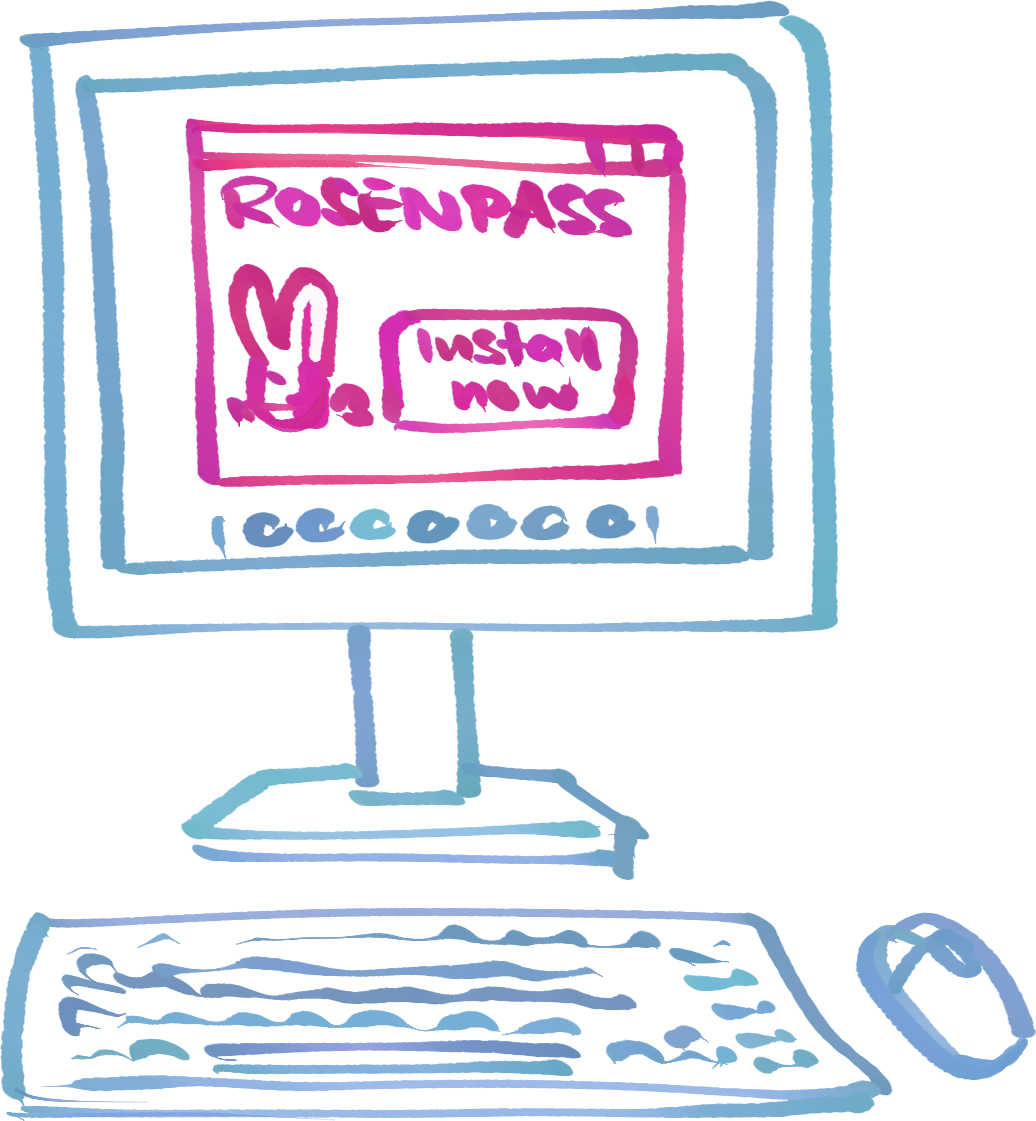
\includegraphics[ width=.92\linewidth]{graphics/Illu-install.png}
    \end{column}
  \end{columns}
\end{frame}
